\chapter{مبانی احتمال و جبر مجموعه ها}

\Q
نشان دهید احتمال هر مجموعه، کمتر از یا مساوی 1 است.

%%%%%%%%%%%%%%%%%%%%%%%%%%%%%%%%%%%%%%

\Q
فرض کنید که برنامه ي نوشته اید که اعداد 1 تا 9 را به صورت کاملا تصادفی در هر بار اجرا در 3 جایگاه (سه رقم) چاپ می کند. احتمال ظاهر شده اعداد با هر سه رقم فرد را محاسبه کنید.

%%%%%%%%%%%%%%%%%%%%%%%%%%%%%%%%%%%%%%

\Q
از کیسه‌ای که دارای 40 مهره سیاه و 60 مهره قرمز است، 20 مهره بر می‌داریم. با چه احتمالی، از این 20 مهره، 5 مهره سیاه و 15 مهره قرمزند؟

%%%%%%%%%%%%%%%%%%%%%%%%%%%%%%%%%%%%%%

\Q
دو کیسه در اختیار داریم. کیسه اول شامل 20 گلوله قرمز و 30 گلوله آبی و دومی شامل 20 گلوله زرد، 30 گلوله آبی و 50 گلوله قرمز است. ابتدا یکی از کیسه ها را به تصادف انتخاب کرده و سپس گلوله‌ای را از داخل آن به تصادف بر می داریم.

الف) با چه احتمالی گلوله انتخاب شده قرمز و از کیسه‌ی 2 است؟

ب) اگر گلوله از کیسه 1 انتخاب شده باشد، با چه احتمالی آبی است؟

پ) اگر گلوله زرد نباشد با چه احتمالی قرمز است؟

ت) اگر گلوله آبی نباشد، با چه احتمالی از کیسه‌ی 2 انتخاب شده است؟

ث) اگر گلوله قرمز یا زرد نباشد، با چه احتمالی از کیسه 2 انتخاب شده است؟

%%%%%%%%%%%%%%%%%%%%%%%%%%%%%%%%%%%%%%

\Q
سه جعبه در اختیار داریم. جعبه‌ی 1 شامل 7 توپ آبی و 3 توپ قرمز، جعبه‌ی 2 شامل 1 توپ آبی، 3 توپ قرمز و 6توپ زرد و جعبه‌ی 3 شامل 7 توپ آبی و 3 توپ زرد هستند. ابتدا یکی از جعبه ها را به تصادف برداشته و سپس توپی از آن جعبه به تصادف بر می‌داریم. اگر توپ بیرون آمده آبی نباشد، با چه احتمالی قرمز است و از جعبه‌ی 1 یا از جعبه‌ی 2 بیرون آمده است؟

%%%%%%%%%%%%%%%%%%%%%%%%%%%%%%%%%%%%%%

\Q
یک عدد دو رقمی را به این صورت می سازیم که هر رقم آن، به صورت تصادفی از بین ارقام 1 تا 9 انتخاب شده باشد. با چه احتمالی، عدد ساخته شده بر 9 بخش پذیر است؟

%%%%%%%%%%%%%%%%%%%%%%%%%%%%%%%%%%%%%%

\Q
سه جعبه داریم که هر یک شامل 10 توپ هستند. در جعبه اول، 3 توپ آبی و 7 توپ قرمز، در جعبه دوم، 3 توپ سفید و 5 توپ آبی و در جعبه سوم، 1 توپ قرمز و 9 توپ سفید هستند. ابتدا یکی از جعبه ها را به تصادف انتخاب کرده و سپس توپی از آن جعبه بیرون می‌کشیم. اگر توپ مورد نظر سفید باشد، با چه احتمالی از جعبه دوم \underline{نیست}؟

%%%%%%%%%%%%%%%%%%%%%%%%%%%%%%%%%%%%%%

\Q
دو نقطه را به تصادف از داخل مربع زیر با طول ضلع 1 انتخاب می کنیم:
 \begin{figure}[h!]
\centering
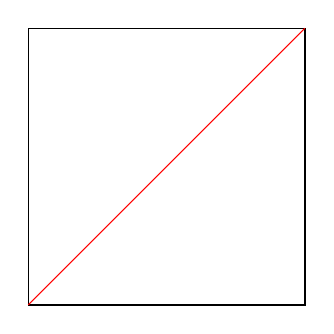
\begin{tikzpicture}
\draw [fill=white,fill opacity=0.5] (0,0)--(0,100pt)--(100pt,100pt)--(100pt,0)--(0,0);
\draw [fill=red,fill opacity=0.5,draw=red] (0,0)--(100pt,100pt);
\end{tikzpicture}
\end{figure}

احتمال اینکه این دو نقطه در دو طرف متفاوت قطر مربع انتخاب شوند و فاصله‌ی هر یک از آنها از قطر نشان داده شده‌ی مربع (قطر قرمز رنگ در شکل) بیش از 0.5 باشد چقدر است؟

%%%%%%%%%%%%%%%%%%%%%%%%%%%%%%%%%%%%%%

\Q
دو جعبه در اختیار داریم. جعبه 1 شامل 10 توپ سفید و 10 توپ آبی و جعبه دوم شامل 20 توپ سفید و 30 توپ قرمز است. ابتدا یکی از جعبه ها را به تصادف انتخاب کرده و سپس از داخل جعبه انتخاب شده، گلوله ای را به تصادف بر می داریم. 

الف) اگر گلوله سفید باشد، با چه احتمالی از جعبه‌ی 2 انتخاب شده است؟

ب) اگر گلوله سفید نباشد، با چه احتمالی قرمز است؟

%%%%%%%%%%%%%%%%%%%%%%%%%%%%%%%%%%%%%%

\Q
یک تاس سالم (که احتمال رخداد هر وجه آن $\frac{1}{6}$ است) را دوبار پرتاب می‌کنیم و نتیجه دوبار پرتاب را در نظر می‌گیریم. اگر واقعه‌ی $A$ معادل حالت هایی باشد که مجموع دو عدد رو آمده کمتر از 5 باشد، و واقعه‌ی $B$ به گونه‌ای باشد که 
$$B=\{(1,4),(2,3),(2,2),(1,2),(3,1)\},$$
در این صورت مقدار احتمال $P(A-B)$ را با بهره گیری از تعریف اصل موضوعی احتمال (کولموگروف) بیابید.

%%%%%%%%%%%%%%%%%%%%%%%%%%%%%%%%%%%%%%

\Q
یک سکه سالم را می اندازیم. اگر رو آمد، تاس سالمی را می اندازیم و عدد رو آمده را یادداشت می‌کنیم و در غیر این صورت، سه تاس را پرتاب کرده و مجموع سه عدد را یادداشت می کنیم. با چه احتمالی، عدد یادداشت شده برابر 4 است؟

%%%%%%%%%%%%%%%%%%%%%%%%%%%%%%%%%%%%%%

\Q
از مجموعه‌ی تمام اعداد دو رقمی بدون ارقام تکراری ای که می‌توان از ارقام 1، 5، 7 و 9 ساخت، عددی را به تصادف بر می گزینیم. با چه احتمالی عدد انتخاب شده، بر 3 بخش پذیر است؟

%%%%%%%%%%%%%%%%%%%%%%%%%%%%%%%%%%%%%%

\Q
کشوری شامل دو استان 1 و 2 است. استان 1 ، شامل 60 مرد و 40 زن و استان 2 شامل 650 زن و 350 مرد است. در استان 1 ، 10 مرد و 10 زن چشم آبی و در استان 2 ، 30 مرد و 20 زن چشم آبی هستند. فردی را به تصادف از این کشور انتخاب می‌کنیم.

الف) اگر این فرد چشم آبی باشد، با چه احتمالی از استان 1 انتخاب شده است؟

ب) اگر این فرد زن باشد، با چه احتمالی از استان 2 انتخاب شده و چشم آبی نیست؟

پ) اگر فرد انتخاب شده مرد باشد، با چه احتمالی چشم آبی است؟

%%%%%%%%%%%%%%%%%%%%%%%%%%%%%%%%%%%%%%

\Q
استانی دارای دو شهر است. شهر 1 دارای 120 مرد و 80 زن و شهر 2 دارای 1000 زن و 800 مرد است. در شهر 1،  50 مرد و 30 زن و در شهر 2، 100 مرد و 150 زن به تب کریمه کنگو مبتلا هستد. فردی را از این استان به تصادف انتخاب می‌کنیم.

الف) با چه احتمالی این فرد، زن سالمی از شهر 1 است؟

ب) اگر فردی که انتخاب می‌کنیم بیمار باشد، با چه احتمالی مردی از شهر 2 است؟

پ) اگر فرد انتخاب شده سالم باشد، احتمال زن بودن او چقدر است؟

%%%%%%%%%%%%%%%%%%%%%%%%%%%%%%%%%%%%%%

\Q
یک سکه سالم را برداشته، آن را سه بار پرتاب می کنیم و نتیجه‌ی سه بار پرتاب را در نظر می‌گیریم. اگر رو آمدن سکه را با H و پشت آمدن را با T نمایش دهیم:

الف) فضای نمونه را بیابید.

ب) این مسئله‌ی احتمال، چند واقعه‌ی محتمل دارد؟ (واقعه طبق تعریف یک زیر مجموعه از فضای نمونه است).

پ) طبق تعریف کلاسیک احتمال، واقعه‌ی اینکه در پرتاب اول و دوم سکه نتیجه یکسان باشد (در پرتاب سوم نتیجه دلخواه است)، با چه احتمالی رخ می دهد؟

%%%%%%%%%%%%%%%%%%%%%%%%%%%%%%%%%%%%%%

\Q
دو مجموعه‌ی 
$A=\{1,4,5\}$
و
$B=\{2,3,4\}$
 را در نظر بگیرید. مجموعه های زیر را به دست آورید.

الف) $A\cap B$
\quad,\quad
ب) $A-B$
\quad,\quad
پ) $A\times B$ (ضرب دکارتی)

ت) اگر 
$C=\{2,5,6\}$
، با محاسبه‌ی مجموعه های 
$(A\cup B)\cap C$
و
$(A\cap C)\cup (B\cap C)$
نشان دهید
$
(A\cup B)\cap C=(A\cap C)\cup (B\cap C)
$.

%%%%%%%%%%%%%%%%%%%%%%%%%%%%%%%%%%%%%%

\Q
به کمک تعریف اصولی احتمال (و با بهره گیری از اصول کولموگروف)، برای هر دو مجموعه‌ی A و B نتیجه بگیرید
$
P(A)=P(A-B)+P(A\cap B)
$.

%%%%%%%%%%%%%%%%%%%%%%%%%%%%%%%%%%%%%%

\Q
در یک کیسه، 5 گلوله‌ی آبی و 3 گلوله‌ی سفید وجود دارد. دو عدد گلوله بر می‌داریم. احتمال این را که یکی از گلوله ها آبی و دیگری سفید باشد، در دو حالت با جایگذاری و بدون جایگذاری به دست آورید (جایگذاری حالتی است که گلوله ای را پس از بیرون آوردن از کیسه و مشاهده‌ی رنگ آن، به کیسه باز گردانیم).

%%%%%%%%%%%%%%%%%%%%%%%%%%%%%%%%%%%%%%

\Q
در نقشه‌ی زیر، از شهر $A$ به شهر $B$ دو مسیر و از $B$ به $C$ یا از $A$ به $C$ یک مسیر وجود دارد. اگر احتمال قطع شدن هر مسیر مستقل از سایرین برابر $p$ باشد، احتمال آن که شخصی بتواند از شهر $A$ به $C$ برود چقدر است؟
\pic{Q2.pdf}{100mm}

%%%%%%%%%%%%%%%%%%%%%%%%%%%%%%%%%%%%%%

\Q
در مبحث مدولاسیون دیجیتال، می‌توان هر سمبل مخابراتی را با تعدادی بیت کد نموده و پس از شکل دهی پالس روی کانال ارسال کرد. فرض کنید یک سمبل مخابراتی از $n$ بیت تشکیل شده باشد. به طور مثال
\eqn{
S_k\equiv (1010001101)_2
}{}
که $k$ اندیس سمبل است و در اینجا سمبل از $10$ بیت تشکیل شده است. این سمبل از یک کانال مخابراتی ارسال و در انتهای کانال دریافت می‌شود. اگر احتمال خرابی هر بیت مستقل از سایرین برابر $p$ باشد، با چه احتمالی سمبل به درستی آشکار \underline{نمی‌شود}؟

%%%%%%%%%%%%%%%%%%%%%%%%%%%%%%%%%%%%%%

\Q
دو تاس را پرتاب می‌کنیم. احتمال اینکه دو عدد رو آمده نسبت به هم اول باشند چقدر است؟

%%%%%%%%%%%%%%%%%%%%%%%%%%%%%%%%%%%%%%

\Q
یک سکه‌ی سالم و یک تاس سالم را با هم پرتاب می کنیم.

الف) احتمال اینکه سکه به رو بیفتد و تاس عدد فرد شود را به دست آورید.

ب) احتمال اینکه سکه به رو بیفتد یا تاس عدد فرد شود را به دست آورید (هر دو باهم نیز می‌توانند رخ دهند!)

%%%%%%%%%%%%%%%%%%%%%%%%%%%%%%%%%%%%%%

\Q
یک تاس را پرتاب می کنیم. اگر مضرب 3 ظاهر شد، نتیجه را یادداشت می کنیم و در غیر این صورت سکه ای را می اندازیم و نتیجه‌ی سکه (پشت یا رو) را می نویسیم.

الف) فضای شدنی این مسئله را بیابید.

ب) با چه احتمالی واقعه‌ی رو آمدن سکه رخ می‌دهد؟

پ) احتمال واقعه‌ی اینکه تاس عدد 1 بیاید یا سکه به پشت ظاهر شود را به دست آورید.

%%%%%%%%%%%%%%%%%%%%%%%%%%%%%%%%%%%%%%

\Q
نقطه‌ای را از داخل مربع زیر بر می‌گزینیم (طول ضلع مربع برابر 2 است).

\begin{figure}[h!]
\centering
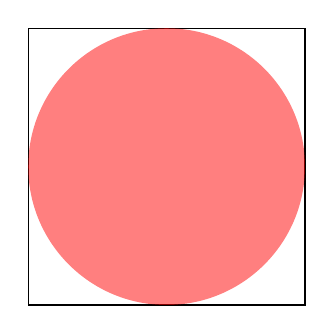
\begin{tikzpicture}
\draw [fill=white,fill opacity=0.5] (0,0)--(0,100pt)--(100pt,100pt)--(100pt,0)--(0,0);
\node [circle,minimum size=100pt,fill=red,fill opacity=0.5] (1) at(50pt,50pt) {};
\end{tikzpicture}
\end{figure}

احتمال اینکه،

الف) نقطه داخل دایره‌ی واحد (نشان داده شده در شکل) بیفتد چقدر است؟

ب) نقطه روی یکی از دو قطر مربع بیفتد چقدر است؟

پ) فاصله‌ی نقطه از هر یک از رأس های مربع بیش از $0.5$ باشد چقدر است؟

%%%%%%%%%%%%%%%%%%%%%%%%%%%%%%%%%%%%%%

\Q
از بین اعداد سه رقمی‌ای که با ترکیب رقم های 0، 1 و  2 می‌توان ساخت (تکرار مجاز است):

الف) چند عدد به 3 بخش پذیرند؟

ب) اگر عددی را به تصادف برگزینیم، با چه احتمالی زوج خواهد بود؟

%%%%%%%%%%%%%%%%%%%%%%%%%%%%%%%%%%%%%%

\Q
در یک جامعه‌ی آماری، نسبت جمعیت زنان بزرگسال، مردان بزرگسال و کودکان به کل جمعیت جامعه به ترتیب برابر $0.37$، $0.43$ و $0.2$ است. در این جامعه، $0.15$ مردان بزرگسال و $0.25$ زنان بزرگسال به نوعی بیماری مبتلا شده اند. فرد بزرگسالی را به تصادف از این جامعه انتخاب می‌کنیم، احتمال بیمار بودن او چقدر است؟

%%%%%%%%%%%%%%%%%%%%%%%%%%%%%%%%%%%%%%

\Q
فرض کنید مجموعه های B و C مستقل و دارای احتمال مثبت باشند. در چه حالتی داریم
$
P(A|B\cap C)=P(A|B)P(A|C)
$
؟

%%%%%%%%%%%%%%%%%%%%%%%%%%%%%%%%%%%%%%

\Q
(کران پایین برای احتمال اجتماع) برای هر دو مجموعه‌ی A و B ثابت کنید
$$
P(A)+P(B)-\frac{1}{4\max\{1-P(A),1-P(B)\}}
\le 
P(A\cup B).
$$

%%%%%%%%%%%%%%%%%%%%%%%%%%%%%%%%%%%%%%

\Q
جعبه‌ی 1 حاوی 1000 لامپ است که 10 درصد آنها خراب هستند. جعبه‌ی 2 نیز حاوی 2000 لامپ است که 5 درصد آنها خراب هستند. از یک جعبه که به طور تصادفی انتخاب شده، دو لامپ بیرون آورده می شوند.

الف) احتمال خرابی هر دو چقدر است؟

ب) اگر هر دو لامپ خراب باشند، با چه احتمالی جعبه‌ی 1 انتخاب شده است؟

%%%%%%%%%%%%%%%%%%%%%%%%%%%%%%%%%%%%%%

\Q
نشان دهید که برای استقلال $n$ رخداد باید 
$2^n-n-1$
 معادله برقرار باشد.

%%%%%%%%%%%%%%%%%%%%%%%%%%%%%%%%%%%%%%

\Q
در یک گل فروشی، 10 گل لاله، 5 نسترن، 3 بنفشه، 2 اقاقیا و 1 رز هلندی وجود دارد. می‌خواهیم دسته گلی شامل 5 گل که همگی به تصادف انتخاب شده باشند، برگزینیم. با چه احتمالی

الف) دسته گل شامل 2 نسترن و 2 بنفشه است؟

ب) دسته گل شامل هیچ گل لاله و بنفشه ای نیست؟

پ) دسته گل شامل حداقل یک گل از هر یک از 4 نوع گل است؟

ت) تمام گلها، از نظر نوع متمایزند؟

(دقت کنید گل های هر نوع با هم فرقی نمی کنند!)

%%%%%%%%%%%%%%%%%%%%%%%%%%%%%%%%%%%%%%

\Q
الف) از یک مجموعه‌ی $n$ عضوي، یک زیر مجموعه به تصادف انتخاب می کنیم. احتمال آن که این زیر مجموعه $k$ عضوي باشد چقدر است؟

ب) به کمک قسمت قبل ثابت کنید
$
\sum_{k=0}^n\binom{n}{k}=2^n
$.

%%%%%%%%%%%%%%%%%%%%%%%%%%%%%%%%%%%%%%

\Q
احتمال اینکه فردی به
\lr{covid-19}
 مبتلا شود، در صورتی که ماسک نزند برابر $70\%$ و در صورتی که ماسک بزند برابر $15\%$ است. اگر این فرد به طور متوسط $5\%$ مواقع ماسک بزند، احتمال کرونا گرفتن او چقدر است؟

%%%%%%%%%%%%%%%%%%%%%%%%%%%%%%%%%%%%%%

\Q
دو تاس می اندازیم و جمع دو عدد رو آمده را یادداشت می کنیم.

الف) احتمال اینکه عدد رو آمده، زوج باشد چقدر است؟

ب) اگر جمع دو عدد رو آمده زوج باشد، با چه احتمالی بیشتر از 8 است؟

%%%%%%%%%%%%%%%%%%%%%%%%%%%%%%%%%%%%%%

\Q
از بین $2^n$ زیرمجموعه‌ی مجموعه‌ی $S=\{1,2,\cdots,n\}$، دو زیر مجموعه به تصادف و مستقل از هم بر می داریم. اگر این دو زیر مجموعه، دارای اشتراک $\{1,2\}$ باشند، احتمال آن که یکی از زیرمجموعه‌ها شامل عضوهای 3، 4 و 5 باشد چقدر است؟ ($n\ge 5$)

%%%%%%%%%%%%%%%%%%%%%%%%%%%%%%%%%%%%%%

\Q
سه جعبه در اختیار داریم. در جعبه‌ی 1، 1000 لامپ موجود است که 3تای آنها معیوبند. جعبه‌ی 2 شامل 10 لامپ است که 3 تای آنها معیوبند و در جعبه‌ی سوم هم 3000 لامپ وجود دارد که همگی سالمند. اگر یکی از این جعبه ها را به تصادف برگزیده و از داخل آن لامپی انتخاب کنیم،

الف) با چه احتمالی لامپ معیوب است؟

ب) اگر لامپ معیوب باشد، با چه احتمالی از جعبه‌ی 2 انتخاب شده است؟

پ) اگر لامپ سالم باشد، با چه احتمالی از یکی از جعبه‌های 1 یا 2 انتخاب شده است؟

%%%%%%%%%%%%%%%%%%%%%%%%%%%%%%%%%%%%%%



\Q
از یک جعبه که دارای $M$ گلوله‌ی سفید و $N-M$ گلوله‌ی سیاه است، $n$ گلوله برداشته می‌شود.

الف)
احتمال آنکه $m$ گلوله از گلوله های برداشته شده سفید باشند در حالت با جایگذاری چقدر است؟

ب)
احتمال آنکه $m$ گلوله از گلوله های برداشته شده سفید باشند در حالت بدون جایگذاری چقدر است؟

ج) اگر بدانیم تمام گلوله های سفید برداشته شده اند، احتمال آنکه دقیقا 2 گلوله‌ی سیاه نیز برداشته شده باشند چقدر است؟

%%%%%%%%%%%%%%%%%%%%%%%%%%%%%%%%%%%%%%

\Q
سکه ای را پرتاب می‌کنیم. اگر رو آمد، دو تاس را پرتاب کرده، جمع دو عدد روی تاس را یادداشت می کنیم. اگر سکه پشت آمد، یک تاس را پرتاب کرده و عدد آنرا یادداشت می کنیم. با چه احتمالی

الف) عدد یادداشت شده برابر 3 است؟
\quad,\quad
ب) عدد یادداشت شده برابر 8 است؟

%%%%%%%%%%%%%%%%%%%%%%%%%%%%%%%%%%%%%%

\Q
موارد زیر را در یک مسئله‌ی احتمالاتی تعریف کنید:

الف) فضای نمونه
\quad,\quad
ب) پیشامد (واقعه)
\quad,\quad
پ) پیشامد (واقعه‌ی) ساده

%%%%%%%%%%%%%%%%%%%%%%%%%%%%%%%%%%%%%%

\Q
آیا فضای نمونه در یک مسئله‌ی احتمالاتی، تنها مجموعه با احتمال یک است؟ پاسخ را برای هر دو حالتی که فضای نمونه متناهی یا نامتناهی باشد شرح دهید و در صورت لزوم، مثال بزنید.

%%%%%%%%%%%%%%%%%%%%%%%%%%%%%%%%%%%%%%

\Q
اگر $A$ فضای نمونه‌ی آزمایش پرتاب سکه با رخدادهای پشت و رو و $B$ فضای نمونه‌ی پرتاب تاس با اعداد طبیعی 1 تا 6 باشد،

الف) حاصلضرب دکارتی $A$ و $B$ (
$A\times B$
)
را به دست آورید. این مجموعه، فضای نمونه‌ی چه آزمایشی است؟

ب) دو زیر مجموعه‌ی 3 عضوی از مجموعه‌ی 
$
A\times B
$
برگزینید که با یکدیگر ناسازگار باشند. آیا می‌توانید همین کار را برای زیرمجموعه‌های 7 عضوی تکرار کنید؟ چرا؟

%%%%%%%%%%%%%%%%%%%%%%%%%%%%%%%%%%%%%%

\Q
با بهره گیری از جبر مجموعه ها و اصول کولموگروف احتمال، نشان دهید اگر $A$، $B$ و $C$ سه مجموعه‌ باشند به طوری که 
$
P(B\cap C)=0
$
، در این صورت
$$
P\left\{
A\cap(B\cup C)
\right\}
=
P\left\{
A\cap B
\right\}
+
P\left\{
A\cap C
\right\}
.
$$

%%%%%%%%%%%%%%%%%%%%%%%%%%%%%%%%%%%%%%

\Q
در یک جامعه، احتمال اینکه فردی به کرونا مبتلا باشد $0.07$ و احتمال آن که به آنفلوآنزا مبتلا باشد $0.19$ است. اگر 20 درصد افراد این جامعه مبتلا به حداقل یکی از این دو بیماری باشند،

الف) چند درصد افراد به هر دو بیماری مبتلا هستند؟

ب) چند درصد افراد \underline{فقط} به کرونا مبتلا هستند؟

%%%%%%%%%%%%%%%%%%%%%%%%%%%%%%%%%%%%%%

\Q
یک عدد از مجموعه‌ی 
$
\{1,2,3,\cdots,10\}
$
به تصادف بر می‌گزینیم. اگر تمام وقایع ساده هم شانس باشند و تعریف کنیم
$
A=\{2,3,5,7\}
$
و
$
B=\{1,3,5,7,9\}
$،

الف) مقدار
$P(A)$
را بیابید.

ب) مجموعه‌های 
$A-B$
و
$A\cap B$
را به دست آورده و مقادیر 
$P(A-B)$
و
$P(A\cap B)$
را بیابید.

پ) تحقیق کنید
$
P(A-B)=P(A)-P(A\cap B)
$.
چه توجیهی برای پاسخ شما وجود دارد؟

%%%%%%%%%%%%%%%%%%%%%%%%%%%%%%%%%%%%%%

\Q
در یک کتابخانه، سه کتاب فیزیک، دو کتاب رمان و چهار کتاب روان شناسی موجود است. مطلوبست تعداد حالات چیدن این کتاب ها در یک قفسه کنار هم چنانچه:

الف) تمام کتابهای هم نوع متمایز باشند (مثلا ترتیب دو کتاب رمان نسبت به هم مهم باشد).

ب) تمام کتابهای هم نوع نامتمایز باشند (مثلا ترتیب دو کتاب رمان نسبت به هم مهم نباشد).

%%%%%%%%%%%%%%%%%%%%%%%%%%%%%%%%%%%%%%

\Q
اعضای یک شرکت شامل 1 مدیرعامل، 2 منشی، 1 حسابدار و 5 نفر از سایر اعضای هیئت مدیره در یک میزگرد دارای 11 صندلی می‌نشینند. مطلوبست تعداد حالاتی که

الف) هر دو منشی کنار هم باشند.

ب) هیچ یک از اعضای هیئت مدیره (به جز مدیرعامل)، مجاور مدیرعامل نباشد.

پ) حسابدار کنار مدیرعامل بنشیند و تمام اعضای هیئت مدیره (به جز مدیرعامل) کنار هم باشند.

(راهنمایی: برای حل این سوال، به تمایز یا عدم تمایز اعضای هیئت مدیره یا منشی ها دقت کنید. آیا منطقی است متمایز باشند یا نباشند؟ همچنین دقت کنید که همواره دو صندلی از میزگرد خالی می مانند و باید در شمارش حالات محاسبه شوند.)

%%%%%%%%%%%%%%%%%%%%%%%%%%%%%%%%%%%%%%

\Q
در کیسه ای، 10 توپ آبی و 7 توپ قرمز موجود است. دو توپ به تصادف و بدون جایگذاری بر می‌داریم.

الف) اگر توپهای همرنگ نامتمایز باشند، تعداد حالات برداشتن دو توپ غیرهمرنگ چقدر است؟

ب) اگر توپهای همرنگ نامتمایز باشند، احتمال برداشتن دو توپ غیرهمرنگ چقدر است؟

پ) اگر توپهای آبی را از 1 تا 10 و توپهای قرمز را از 1 تا 7 شماره گذاری کنیم، احتمال آنکه توپ آبی شماره 4 و توپ آبی شماره 3 برداشته شود چقدر است؟

ت) اگر توپهای آبی را از 1 تا 10 و توپهای قرمز را از 1 تا 7 شماره گذاری کنیم، آیا احتمال برداشتن دو توپ غیرهمرنگ، با مقدار بدست آمده در قسمت الف تفاوت می‌کند؟ توضیح دهید.

%%%%%%%%%%%%%%%%%%%%%%%%%%%%%%%%%%%%%%

\Q
قسمتهای ب)، پ) و ت) مسئله‌ی پیش را با فرض داشتن جایگذاری حل کنید؛ یعنی زمانی که توپ اول را برداشتیم، رنگ آن را یادداشت کرده، آنرا به کیسه بازگردانده و سپس توپ دوم را بر می‌داریم.

%%%%%%%%%%%%%%%%%%%%%%%%%%%%%%%%%%%%%%

\Q
نقطه‌ای را از داخل مربع به تصادف انتخاب می‌کنیم. احتمال آنکه فاصله‌ی این نقطه تا مرکز مربع، از فاصله‌ی این نقطه تا هر یک از رئوس مربع بیشتر باشد چقدر است؟

%%%%%%%%%%%%%%%%%%%%%%%%%%%%%%%%%%%%%%

\Q
از مجموعه‌ی زیرمجموعه‌های مجموعه‌ی
$
\{1,2,3,\cdots,n\}
$
، دو زیرمجموعه‌‌‌ی متمایز به تصادف انتخاب می‌کنیم. با چه احتمالی، این دو زیرمجموعه ناسازگارند؟

%%%%%%%%%%%%%%%%%%%%%%%%%%%%%%%%%%%%%%

\Q
الف) در یک صفحه‌ی شطرنجی 8 در 8، یک مهره‌ی رخ سفید به تصادف در یکی از خانه‌های این صفحه قرار می‌گیرد. سپس، یک مهره‌ی رخ سیاه را به تصادف در یکی از خانه‌های این صفحه قرار می‌دهیم. با چه احتمالی، رخ سیاه در معرض حمله‌ی رخ سفید قرار می‌گیرد؟ (حرکت رخ، به صورت افقی یا عمودی در صفحه است)

ب) یک مهره‌ی شاه سفید، در یکی از گوشه‌های یک صفحه‌ی شطرنجی 8 در 8 قرار دارد. دو رخ سیاه به تصادف در دو خانه‌ی این صفحه قرار می‌گیرند. با چه احتمالی، شاه سفید مات می‌شود؟ (مات شدن شاه، زمانی اتفاق می‌افتد که نوبت حرکت شاه بوده و با هر حرکت، در معرض حمله‌ی یکی از مهره‌های دشمن قرار گیرد)

\begin{figure}[h]
\centering
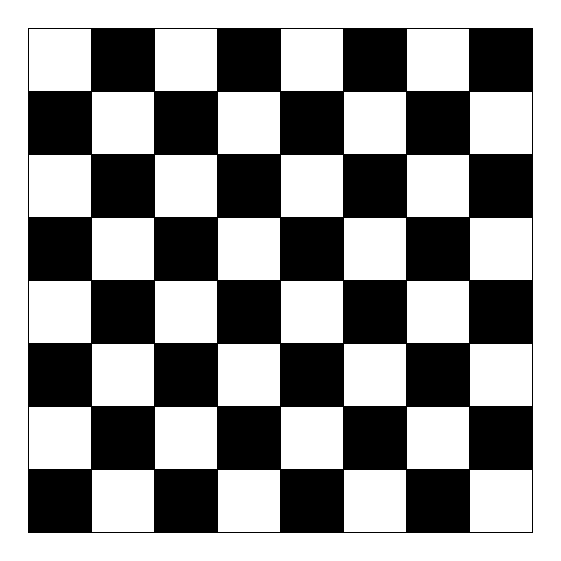
\begin{tikzpicture}
\filldraw[fill=black](-3.2,-3.2)--(-2.4000000000000004,-3.2)--(-2.4000000000000004,-2.4000000000000004)--(-3.2,-2.4000000000000004)--(-3.2,-3.2);
\filldraw[fill=white](-3.2,-2.4000000000000004)--(-2.4000000000000004,-2.4000000000000004)--(-2.4000000000000004,-1.6000000000000003)--(-3.2,-1.6000000000000003)--(-3.2,-2.4000000000000004);
\filldraw[fill=black](-3.2,-1.6)--(-2.4000000000000004,-1.6)--(-2.4000000000000004,-0.8)--(-3.2,-0.8)--(-3.2,-1.6);
\filldraw[fill=white](-3.2,-0.8)--(-2.4000000000000004,-0.8)--(-2.4000000000000004,0.0)--(-3.2,0.0)--(-3.2,-0.8);
\filldraw[fill=black](-3.2,0.0)--(-2.4000000000000004,0.0)--(-2.4000000000000004,0.8)--(-3.2,0.8)--(-3.2,0.0);
\filldraw[fill=white](-3.2,0.8)--(-2.4000000000000004,0.8)--(-2.4000000000000004,1.6)--(-3.2,1.6)--(-3.2,0.8);
\filldraw[fill=black](-3.2,1.6)--(-2.4000000000000004,1.6)--(-2.4000000000000004,2.4000000000000004)--(-3.2,2.4000000000000004)--(-3.2,1.6);
\filldraw[fill=white](-3.2,2.4000000000000004)--(-2.4000000000000004,2.4000000000000004)--(-2.4000000000000004,3.2)--(-3.2,3.2)--(-3.2,2.4000000000000004);
\filldraw[fill=white](-2.4000000000000004,-3.2)--(-1.6000000000000003,-3.2)--(-1.6000000000000003,-2.4000000000000004)--(-2.4000000000000004,-2.4000000000000004)--(-2.4000000000000004,-3.2);
\filldraw[fill=black](-2.4000000000000004,-2.4000000000000004)--(-1.6000000000000003,-2.4000000000000004)--(-1.6000000000000003,-1.6000000000000003)--(-2.4000000000000004,-1.6000000000000003)--(-2.4000000000000004,-2.4000000000000004);
\filldraw[fill=white](-2.4000000000000004,-1.6)--(-1.6000000000000003,-1.6)--(-1.6000000000000003,-0.8)--(-2.4000000000000004,-0.8)--(-2.4000000000000004,-1.6);
\filldraw[fill=black](-2.4000000000000004,-0.8)--(-1.6000000000000003,-0.8)--(-1.6000000000000003,0.0)--(-2.4000000000000004,0.0)--(-2.4000000000000004,-0.8);
\filldraw[fill=white](-2.4000000000000004,0.0)--(-1.6000000000000003,0.0)--(-1.6000000000000003,0.8)--(-2.4000000000000004,0.8)--(-2.4000000000000004,0.0);
\filldraw[fill=black](-2.4000000000000004,0.8)--(-1.6000000000000003,0.8)--(-1.6000000000000003,1.6)--(-2.4000000000000004,1.6)--(-2.4000000000000004,0.8);
\filldraw[fill=white](-2.4000000000000004,1.6)--(-1.6000000000000003,1.6)--(-1.6000000000000003,2.4000000000000004)--(-2.4000000000000004,2.4000000000000004)--(-2.4000000000000004,1.6);
\filldraw[fill=black](-2.4000000000000004,2.4000000000000004)--(-1.6000000000000003,2.4000000000000004)--(-1.6000000000000003,3.2)--(-2.4000000000000004,3.2)--(-2.4000000000000004,2.4000000000000004);
\filldraw[fill=black](-1.6,-3.2)--(-0.8,-3.2)--(-0.8,-2.4000000000000004)--(-1.6,-2.4000000000000004)--(-1.6,-3.2);
\filldraw[fill=white](-1.6,-2.4000000000000004)--(-0.8,-2.4000000000000004)--(-0.8,-1.6000000000000003)--(-1.6,-1.6000000000000003)--(-1.6,-2.4000000000000004);
\filldraw[fill=black](-1.6,-1.6)--(-0.8,-1.6)--(-0.8,-0.8)--(-1.6,-0.8)--(-1.6,-1.6);
\filldraw[fill=white](-1.6,-0.8)--(-0.8,-0.8)--(-0.8,0.0)--(-1.6,0.0)--(-1.6,-0.8);
\filldraw[fill=black](-1.6,0.0)--(-0.8,0.0)--(-0.8,0.8)--(-1.6,0.8)--(-1.6,0.0);
\filldraw[fill=white](-1.6,0.8)--(-0.8,0.8)--(-0.8,1.6)--(-1.6,1.6)--(-1.6,0.8);
\filldraw[fill=black](-1.6,1.6)--(-0.8,1.6)--(-0.8,2.4000000000000004)--(-1.6,2.4000000000000004)--(-1.6,1.6);
\filldraw[fill=white](-1.6,2.4000000000000004)--(-0.8,2.4000000000000004)--(-0.8,3.2)--(-1.6,3.2)--(-1.6,2.4000000000000004);
\filldraw[fill=white](-0.8,-3.2)--(0.0,-3.2)--(0.0,-2.4000000000000004)--(-0.8,-2.4000000000000004)--(-0.8,-3.2);
\filldraw[fill=black](-0.8,-2.4000000000000004)--(0.0,-2.4000000000000004)--(0.0,-1.6000000000000003)--(-0.8,-1.6000000000000003)--(-0.8,-2.4000000000000004);
\filldraw[fill=white](-0.8,-1.6)--(0.0,-1.6)--(0.0,-0.8)--(-0.8,-0.8)--(-0.8,-1.6);
\filldraw[fill=black](-0.8,-0.8)--(0.0,-0.8)--(0.0,0.0)--(-0.8,0.0)--(-0.8,-0.8);
\filldraw[fill=white](-0.8,0.0)--(0.0,0.0)--(0.0,0.8)--(-0.8,0.8)--(-0.8,0.0);
\filldraw[fill=black](-0.8,0.8)--(0.0,0.8)--(0.0,1.6)--(-0.8,1.6)--(-0.8,0.8);
\filldraw[fill=white](-0.8,1.6)--(0.0,1.6)--(0.0,2.4000000000000004)--(-0.8,2.4000000000000004)--(-0.8,1.6);
\filldraw[fill=black](-0.8,2.4000000000000004)--(0.0,2.4000000000000004)--(0.0,3.2)--(-0.8,3.2)--(-0.8,2.4000000000000004);
\filldraw[fill=black](0.0,-3.2)--(0.8,-3.2)--(0.8,-2.4000000000000004)--(0.0,-2.4000000000000004)--(0.0,-3.2);
\filldraw[fill=white](0.0,-2.4000000000000004)--(0.8,-2.4000000000000004)--(0.8,-1.6000000000000003)--(0.0,-1.6000000000000003)--(0.0,-2.4000000000000004);
\filldraw[fill=black](0.0,-1.6)--(0.8,-1.6)--(0.8,-0.8)--(0.0,-0.8)--(0.0,-1.6);
\filldraw[fill=white](0.0,-0.8)--(0.8,-0.8)--(0.8,0.0)--(0.0,0.0)--(0.0,-0.8);
\filldraw[fill=black](0.0,0.0)--(0.8,0.0)--(0.8,0.8)--(0.0,0.8)--(0.0,0.0);
\filldraw[fill=white](0.0,0.8)--(0.8,0.8)--(0.8,1.6)--(0.0,1.6)--(0.0,0.8);
\filldraw[fill=black](0.0,1.6)--(0.8,1.6)--(0.8,2.4000000000000004)--(0.0,2.4000000000000004)--(0.0,1.6);
\filldraw[fill=white](0.0,2.4000000000000004)--(0.8,2.4000000000000004)--(0.8,3.2)--(0.0,3.2)--(0.0,2.4000000000000004);
\filldraw[fill=white](0.8,-3.2)--(1.6,-3.2)--(1.6,-2.4000000000000004)--(0.8,-2.4000000000000004)--(0.8,-3.2);
\filldraw[fill=black](0.8,-2.4000000000000004)--(1.6,-2.4000000000000004)--(1.6,-1.6000000000000003)--(0.8,-1.6000000000000003)--(0.8,-2.4000000000000004);
\filldraw[fill=white](0.8,-1.6)--(1.6,-1.6)--(1.6,-0.8)--(0.8,-0.8)--(0.8,-1.6);
\filldraw[fill=black](0.8,-0.8)--(1.6,-0.8)--(1.6,0.0)--(0.8,0.0)--(0.8,-0.8);
\filldraw[fill=white](0.8,0.0)--(1.6,0.0)--(1.6,0.8)--(0.8,0.8)--(0.8,0.0);
\filldraw[fill=black](0.8,0.8)--(1.6,0.8)--(1.6,1.6)--(0.8,1.6)--(0.8,0.8);
\filldraw[fill=white](0.8,1.6)--(1.6,1.6)--(1.6,2.4000000000000004)--(0.8,2.4000000000000004)--(0.8,1.6);
\filldraw[fill=black](0.8,2.4000000000000004)--(1.6,2.4000000000000004)--(1.6,3.2)--(0.8,3.2)--(0.8,2.4000000000000004);
\filldraw[fill=black](1.6,-3.2)--(2.4000000000000004,-3.2)--(2.4000000000000004,-2.4000000000000004)--(1.6,-2.4000000000000004)--(1.6,-3.2);
\filldraw[fill=white](1.6,-2.4000000000000004)--(2.4000000000000004,-2.4000000000000004)--(2.4000000000000004,-1.6000000000000003)--(1.6,-1.6000000000000003)--(1.6,-2.4000000000000004);
\filldraw[fill=black](1.6,-1.6)--(2.4000000000000004,-1.6)--(2.4000000000000004,-0.8)--(1.6,-0.8)--(1.6,-1.6);
\filldraw[fill=white](1.6,-0.8)--(2.4000000000000004,-0.8)--(2.4000000000000004,0.0)--(1.6,0.0)--(1.6,-0.8);
\filldraw[fill=black](1.6,0.0)--(2.4000000000000004,0.0)--(2.4000000000000004,0.8)--(1.6,0.8)--(1.6,0.0);
\filldraw[fill=white](1.6,0.8)--(2.4000000000000004,0.8)--(2.4000000000000004,1.6)--(1.6,1.6)--(1.6,0.8);
\filldraw[fill=black](1.6,1.6)--(2.4000000000000004,1.6)--(2.4000000000000004,2.4000000000000004)--(1.6,2.4000000000000004)--(1.6,1.6);
\filldraw[fill=white](1.6,2.4000000000000004)--(2.4000000000000004,2.4000000000000004)--(2.4000000000000004,3.2)--(1.6,3.2)--(1.6,2.4000000000000004);
\filldraw[fill=white](2.4000000000000004,-3.2)--(3.2,-3.2)--(3.2,-2.4000000000000004)--(2.4000000000000004,-2.4000000000000004)--(2.4000000000000004,-3.2);
\filldraw[fill=black](2.4000000000000004,-2.4000000000000004)--(3.2,-2.4000000000000004)--(3.2,-1.6000000000000003)--(2.4000000000000004,-1.6000000000000003)--(2.4000000000000004,-2.4000000000000004);
\filldraw[fill=white](2.4000000000000004,-1.6)--(3.2,-1.6)--(3.2,-0.8)--(2.4000000000000004,-0.8)--(2.4000000000000004,-1.6);
\filldraw[fill=black](2.4000000000000004,-0.8)--(3.2,-0.8)--(3.2,0.0)--(2.4000000000000004,0.0)--(2.4000000000000004,-0.8);
\filldraw[fill=white](2.4000000000000004,0.0)--(3.2,0.0)--(3.2,0.8)--(2.4000000000000004,0.8)--(2.4000000000000004,0.0);
\filldraw[fill=black](2.4000000000000004,0.8)--(3.2,0.8)--(3.2,1.6)--(2.4000000000000004,1.6)--(2.4000000000000004,0.8);
\filldraw[fill=white](2.4000000000000004,1.6)--(3.2,1.6)--(3.2,2.4000000000000004)--(2.4000000000000004,2.4000000000000004)--(2.4000000000000004,1.6);
\filldraw[fill=black](2.4000000000000004,2.4000000000000004)--(3.2,2.4000000000000004)--(3.2,3.2)--(2.4000000000000004,3.2)--(2.4000000000000004,2.4000000000000004);
\end{tikzpicture}
\end{figure}

%%%%%%%%%%%%%%%%%%%%%%%%%%%%%%%%%%%%%%

\Q
یک سکه‌ی سالم را پرتاب می‌کنیم. اگر رو بیاید، یک تاس را پرتاب کرده و عدد روی آن را یادداشت می‌کنیم. اگر سکه پشت بیاید، دو تاس را پرتاب کرده و جمع اعداد دو تاس را یادداشت می‌کنیم. احتمال آنکه عدد رو آمده برابر $n$ باشد چقدر است؟ (
$
2\le n\le 12
$
)

%%%%%%%%%%%%%%%%%%%%%%%%%%%%%%%%%%%%%%

\Q
از کیسه‌ای که شامل 7 توپ سیاه و 10 توپ سفید است، 3 توپ به تصادف بیرون می‌آوریم. سپس از بین 3 توپ بیرون آمده، یکی را به تصادف بر می‌گزینیم. اگر بدانیم حداقل یک توپ از 3 توپ بیرون آمده سیاه است، احتمال آنکه توپ انتخابی از بین این 3 توپ، سفید باشد چقدر است؟

%%%%%%%%%%%%%%%%%%%%%%%%%%%%%%%%%%%%%%

\Q
دو کیسه در اختیار داریم. کیسه‌ی 1 شامل 7 توپ سیاه و 10 توپ سفید و کیسه‌ی 2 شامل 4 توپ سیاه، 2 توپ سفید و 3 توپ قرمز است. ابتدا یکی از کیسه‌ها را به تصادف انتخاب کرده و سپس، توپی از آن به تصادف بیرون می‌آوریم. اگر بدانیم توپ انتخابی سفید نیست، با چه احتمالی از کیسه‌ی 2 انتخاب شده است؟

%%%%%%%%%%%%%%%%%%%%%%%%%%%%%%%%%%%%%%

\Q
فرض کنید در نقشه‌ی زیر قصد داریم از شهر A به شهر Z برویم. هر یک از 7 لینک نقشه‌ی زیر، با احتمال $p$ مستقل از سایر لینک ها سالم هستند. احتمال آن که مسیر سالمی از A تا Z وجود داشته باشد چقدر است؟

\begin{figure}[h]
\Large
\centering
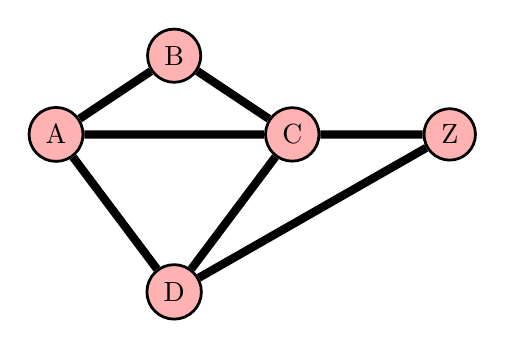
\begin{tikzpicture}
\node [draw=black,fill=white!70!red,circle,line width=1] (A) at (0,0) {A};
\node [draw=black,fill=white!70!red,circle,line width=1] (B) at (1.5,1) {B};
\node [draw=black,fill=white!70!red,circle,line width=1] (C) at (3,0) {C};
\node [draw=black,fill=white!70!red,circle,line width=1] (D) at (1.5,-2) {D};
\node [draw=black,fill=white!70!red,circle,line width=1] (Z) at (5,0) {Z};
\draw[line width=3]
(A)--(B)
(B)--(C)
(C)--(Z)
(A)--(C)
(A)--(D)
(D)--(C)
(D)--(Z)
;
\end{tikzpicture}
\end{figure}

%%%%%%%%%%%%%%%%%%%%%%%%%%%%%%%%%%%%%%

\Q
از کیسه‌ای که شامل 5 مهره سیاه، 8 مهره سفید و 1 مهره قرمز است، دو توپ به تصادف بیرون می‌آوریم. احتمال آنکه هر دو توپ همرنگ باشند چقدر است؟

%%%%%%%%%%%%%%%%%%%%%%%%%%%%%%%%%%%%%%

\Q
دو جعبه از لامپ‌ها در اختیار داریم. جعبه‌ی اول، دارای 1000 لامپ است که $1\%$ آنها سالمند. جعبه‌ی دوم، دارای 10000 لامپ است که $95\%$ آنها سالم اند. یکی از جعبه‌ها را به تصادف انتخاب کرده و دو لامپ بیرون می‌کشیم. احتمال آن که هر دو لامپ از جعبه‌ی 1 انتخاب شده باشند چقدر است اگر

الف) هر دو لامپ خراب باشند.

ب) اگر یکی از لامپ ها سالم و دیگری خراب باشد.